% ------------------------------------------------------------------------------
% The implemtations shows specifically how your research was conducted.
% All the impementation details and practical tests can be listed.
% ------------------------------------------------------------------------------

\opt{never}{\addbibresource{03-tail/bibliography.bib}} % to make citation found in most IDE

\chapter{Implementation}
\label{chap:implementation}

% -- Your text goes here --
The implementation sets out the concrete realisation of the reference architecture, detailing the tools used to automate the deployment of the \gls{cloud_infrastructure} and the integration of the embedded systems. Particular attention is paid to the in-depth description of the automated pipeline. The various applications that accompany this architecture are also highlighted.

\minitoc
\newpage

% ------------------------------------------------------------------------------
\section{Reference architecture}

% -- Your text goes here --
\subsection{\Gls{cloud_infrastructure}}
An \acrfull{iac} tool was selected to orchestrate the efficient deployment of the \gls{cloud_infrastructure} on \gls{aws}, and Pulumi was chosen because of its choice of programming language, in this case Python. The use of the same programming language for the implementation of applications and the description of \gls{aws} resources provides consistency within the project.

Integrating Pulumi is simple. The resources required are described in Python files. The deployment is managed by the Pulumi \acrshort{cli}, which records the state of the infrastructure in an Amazon S3 compartment. This compartment is located in the same \gls{aws} account as the infrastructure, using Amazon S3 to store the state rather than the default Pulumi \Gls{cloud} platform, thus eliminating external dependencies. Figure \ref{fig:pulumi_overview} shows an overview of this part of the implementation.
\begin{center}
    \begingroup
    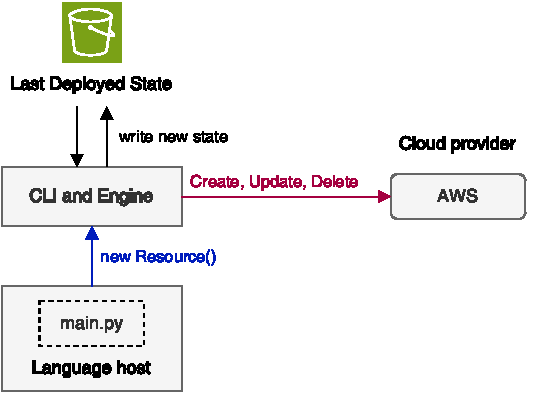
\includegraphics[width=.7\columnwidth]{implementation/pulumi_overview.pdf}
    \captionof{figure}{Overview of Pulumi's integration into the reference architecture}
    \label{fig:pulumi_overview}
    \endgroup
\end{center}
This \gls{cloud_infrastructure} part is implemented in a specific folder as follows :
\begin{center}
    \usemintedstyle{pastie}
    \begin{minted}
    [
    fontsize=\scriptsize
    ]{text}
    cloud-infrastructure
        ├── Pulumi.yaml
        ├── Pulumi.dev.yaml
        ├── Pulumi.prod.yaml
        ├── main.py
        ├── iam.py
        └── requirements.txt
    \end{minted}
\end{center}
The main configuration file for the Pulumi tool, \textit{Pulumi.yaml}, includes crucial information such as the name of the stack and the programming language used, in this case Python.

This implementation aims to facilitate the deployment of two distinct infrastructures, namely the development environment and the production environment. Therefore, two additional configuration files, \textit{Pulumi.dev.yaml} and \textit{Pulumi.prod.yaml}, are present to differentiate these two environments. \textit{Pulumi.dev.yaml} contains parameters such as the development account ID and the deployment region, while \textit{Pulumi.prod.yaml} includes the same parameters with production-specific values. The identifiers of the \gls{aws} accounts must be different.

The Python files \textit{main.py} and \textit{iam.py} detail the description of the resources to be deployed. \textit{iam.py} focuses on IAM roles and policies, while \textit{main.py} mainly covers resources related to \acrshort{iot} and other resources.

Finally, the \textit{requirements.txt} file lists the Pulumi libraries to be installed, including the main Pulumi library, which is essential for all \acrshort{iac} projects.

In terms of the Pulumi libraries used, \gls{aws} Native, a new preview, uses the \gls{aws} \Gls{cloud} Control API to manage and provision \gls{aws} resources, generally aligning with the latest \gls{aws} features as they are released. The resources available in this library are based on those defined in the \gls{aws} CloudFormation registry. In addition, \gls{aws} Classic is another library that is used to fill in resources that are not yet available in \gls{aws} Native. This library uses the \gls{aws} SDK to manage and provision these resources.


\subsection{Embedded systems integration}
\subsubsection{\gls{aws} \acrshort{iot} Greengrass}
Integrating embedded systems with the \gls{aws} ecosystem is crucial to reaping the full benefits of \hyperref[subsec:cloudcomputing]{cloud computing}. To this end, \gls{aws} \acrshort{iot} Greengrass was chosen, a powerful solution that facilitates the execution of local processing on \acrshort{iot} devices, while enabling seamless interaction with \gls{aws} \gls{cloud} services. \gls{aws} defined this solution as follows :
\begin{quote}
    \textit{\gls{aws} \acrshort{iot} Greengrass is an open source \acrfull{iot} edge runtime and \gls{cloud} service that helps you build, deploy and manage \acrshort{iot} applications on your devices. You can use \gls{aws} \acrshort{iot} Greengrass to build software that enables your devices to act locally on the data that they generate, run predictions based on machine learning models, and filter and aggregate device data. \gls{aws} \acrshort{iot} Greengrass enables your devices to collect and analyze data closer to where that data is generated, react autonomously to local events, and communicate securely with other devices on the local network. Greengrass devices can also communicate securely with \gls{aws} \acrshort{iot} Core and export \acrshort{iot} data to the \gls{aws} Cloud. You can use \gls{aws} \acrshort{iot} Greengrass to build edge applications using pre-built software modules, called components, that can connect your edge devices to \gls{aws} services or third-party services. You can also use \gls{aws} \acrshort{iot} Greengrass to package and run your software using Lambda functions, Docker containers, native operating system processes, or custom runtimes of your choice. \cite{aws_iot_greengrass}}\\
\end{quote}
In this implementation, \gls{aws} \acrshort{iot} Greengrass Core software is deployed on embedded systems, acting as an intelligent hub that manages interactions with the \gls{aws} \gls{cloud}. It adapts perfectly to Linux OS. Greengrass components, encapsulating the necessary code, dependencies and resources, are then deployed automatically using mechanisms such as \gls{aws} \acrshort{iot} Greengrass Deployment.

A component must be installed. \textit{Greengrass nucleus} (aws.greengrass.Nucleus) is a mandatory component and the minimum requirement for running \gls{aws} \acrshort{iot} Greengrass Core software on a device. It is configurable to customize and update the \gls{aws} \acrshort{iot} Greengrass Core software \acrlong{ota}.

\subsubsection{Communication}
In this project, components running on an embedded system use the \gls{aws} \acrshort{iot} Greengrass Core \acrfull{ipc} library, available in the \gls{aws} \acrshort{iot} Device SDK, to exchange data with the \gls{aws} \acrshort{iot} Greengrass nucleus and other Greengrass components. The \acrshort{ipc} interface supports the \acrlong{mqtt} communication protocol.

Publish/subscribe messaging allows messages to be sent and received in topics. Components can publish messages in topics to communicate with other components, and those who have subscribed to the topic can act on messages received. In this case, the communication is local to the \acrshort{iot} device.

The \acrshort{ipc} interface also facilitates the sending and receiving of \acrshort{mqtt} messages between \gls{aws} \acrshort{iot} Greengrass and \gls{aws} \acrshort{iot} Core. Components can publish messages to \gls{aws} \acrshort{iot} Core and subscribe to topics to react to \acrshort{mqtt} messages from other sources.